%%
%  ******************************************************************************
%  * #file    Szablon_raportu_EN_Latex.tex
%  * #author  Adrian Wójcik   adrian.wojcik(at)put.poznan.pl
%  *          
%  * #commit  Patryk Kościk   koscikpatryk(at)gmail.com
%  *          Modified the template for Projekt przejsciowy purposes          
%  *          
%  * #version 1.0
%  * #date    09-Mar-2022
%  * #brief   PROJPRZEJ
%  *
%  ******************************************************************************
%%  
\documentclass[11pt, a4paper]{article}

\usepackage{SM_template}

% Wypełnijcie te dyrektywy zgodnie z waszym tematem
% \lab      -> NAZWA CZUJNIKA, np.: 'DHT22'
% \comment  -> Króciutki opis co to, np.: 'Cyfrowy budżetowy czujnik temperatury'
%
\lab{Moduł KY-017}
\comment{Czujnik przechylenia - przełącznik rtęciowy}

% Absolutny zakaz dotykania tego tutaj bo jak dotkiecie to coś jebnie
\university{Politechnika Poznańska}
\faculty{Wydział Automatyki, Robotyki i Elektrotechniki}
\institute{Instytut Robotyki i Inteligencji Maszynowej}
\department{Zakład Sterowania i Elektroniki Przemysłowej}
\addbibresource{bib/KY-017.bib}
\nocite{*}


%%
%
% Początek dokumentu
%
%%
\begin{document}

%% Strona tytułowa %%
\mainpage{{KY-017/ky017.jpeg}}
\newpage

\section*{Opis elementu} \addcontentsline{toc}{section}{Wstęp}
Sensor wykrycia przechylenia KY-017, to prosty łącznik elektryczny, wykorzystujący kluczowe cechy
rtęci, takie jak jej płynność w temperaturach pokojowych, do określenia orientacji czujnika w przestrzeni.

Składa się on z przełącznika rtęciowego, rezystora podciągającego oraz diody
LED sygnalizujące zamknięcie się przełącznika, czyli obrót modułu.

\vspace{0.5cm}
\begin{figure}[h]
\centering
\begin{subfigure}{.5\textwidth}
  \centering
  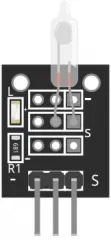
\includegraphics[width=.3\linewidth]{fig/KY-017/zdj_modułu/obr.jpg}
\end{subfigure}%
\begin{subfigure}{.5\textwidth}
  \centering
  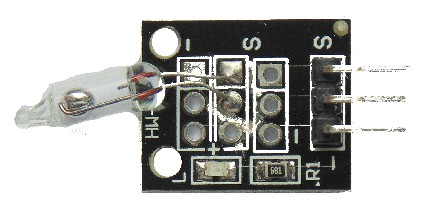
\includegraphics[width=.8\linewidth]{fig/KY-017/zdj_modułu/img4.jpg}
\end{subfigure}
\caption{Ilustracja oraz zdjęcie modułu}
\label{fig:test}
\end{figure}
\vspace{0.5cm}

\subsection{Zasada działania}
Sercem czujnika jest element przełącznika rtęciowego  (zdj.\ref{fig:sub1}), który wykorzystując fakt
przewodnictwa prądowego oraz stanu skupienia cieczy w temperaturach pokojowych (zdj. \ref{fig:sub2}).

Czujnik przechylony o pewny kąt pozwala cieczy zewrzeć dwa metalowe zestyki, funkcjonujące w konfiguracji
takiej identycznej do zwykłego przycisku.

\vspace{0.25cm}
\begin{figure}[h]
\centering
\begin{subfigure}{.5\textwidth}
  \centering
  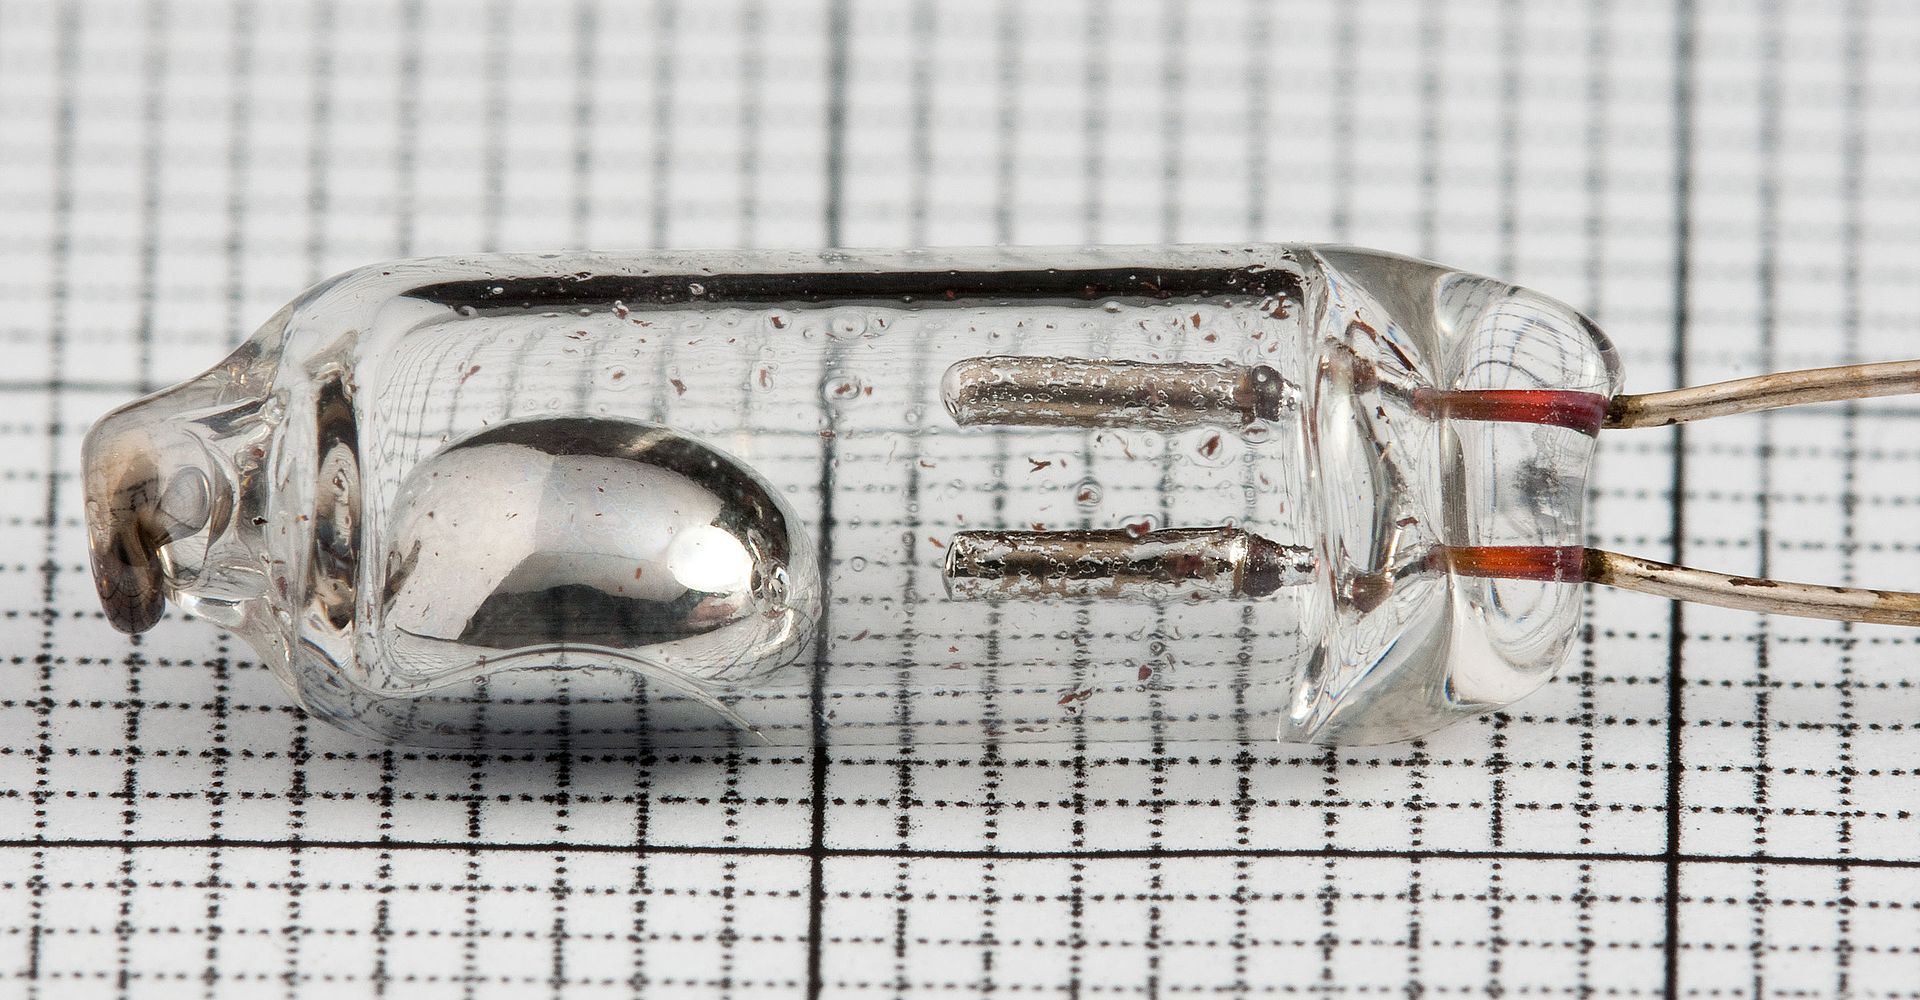
\includegraphics[width=.6\linewidth]{fig/KY-017/zasada_dzialania/Mercury_Switch_without_housing.jpg}
  \caption{Zdjęcie elementu przełącznika rtęciowego}
  
  \label{fig:sub1}
\end{subfigure}%
\begin{subfigure}{.5\textwidth}
  \centering
  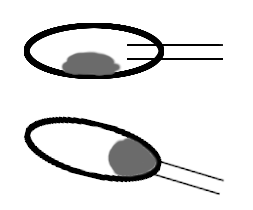
\includegraphics[width=.4\linewidth]{fig/KY-017/zasada_dzialania/otw.png}
  \caption{Przełącznik - otwarty oraz zamknięty}
  \label{fig:sub2}
\end{subfigure}
\caption{Dwa przyciski}
\label{fig:test}
\end{figure}
\vspace{0.25cm}



\subsection{Zastosowania}
Czujnik pomimo swojej prostoty możemy znaleźć w wielu urządzeniach między innymi:

\begin{itemize}
    \item Maszyny pracujące w ciężkim terenie $\rightarrow$ wykrywanie przechylenia, wzniesienie alarmu
    \item Elementy awioniki lotniczej $\rightarrow$ utrzymanie osi żyroskopu w pionie
    \item Do roku 2000 były powszechnie stosowane w przemyśle motoryzacyjnym $\rightarrow$ np. wykrycie otworzenia klapy bagażnika
\end{itemize}
\vspace{0.5cm}

\newpage

\section{Implementacja czujnika}
Ogólny schemat elektryczny modułu KY-021 przedstawiono poniżej. Należy zwrócić uwagę na to że czujnik
ten, ze względu na obecność diody LED, jest spolaryzowany. Oznacza to że nie możemy dowolnie zamieniać
pinu \texttt{GND} oraz \texttt{Vcc}.

\subsection{Połączenie fizyczne}

\vspace{0.5cm}
\begin{figure}[h!]
    \centering
    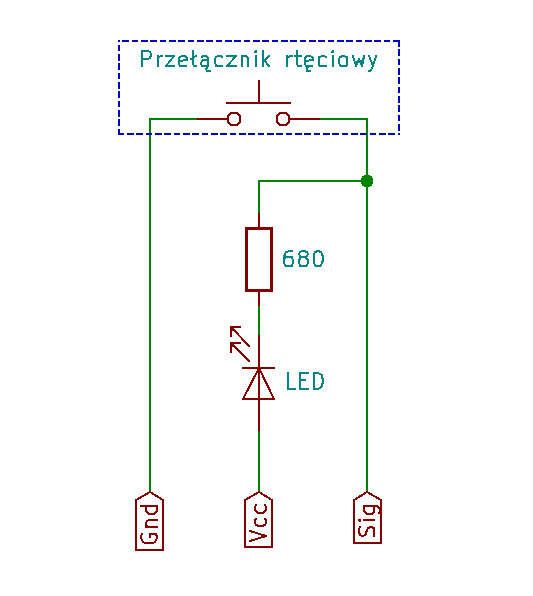
\includegraphics[width=8cm]{fig/KY-017/polaczenie_modulu/kicad.png}
    \caption{Schemat modułu z wyprowadzeniami}
    \label{fig:schemat_z_wyp}
\end{figure}
\vspace{0.5cm}

\vspace{0.5cm}
\begin{table}[h!]
    \centering
    \begin{tabular}{|c|c|c|c|} 
        \hline
        \multicolumn{2}{|c|}{NUCELO-F746ZG} & \multicolumn{2}{c|}{SENSOR}  \\ 
        \hline
        Etykieta & Port i numer pinu       & Nr pinu & Etykieta           \\ 
        \hline
        GND     & -                         & 1       & Gnd              \\
        5V      & CN8-9                     & 2       & Vcc              \\
        D7      & PF13                      & 3       & Sig             \\
        \hline
    \end{tabular}
    \caption{Tabela połączeń czujnika z mikrokontrolerem}
\end{table}
\vspace{0.5cm}

\newpage

\subsection{Kongiuracja IOC}
W oprogramowaniu \texttt{CubeIDE} skonfigurowano następujące peryferia mikrokontrolera.

\vspace{0.5cm}
\begin{figure}[h!]
    \centering
    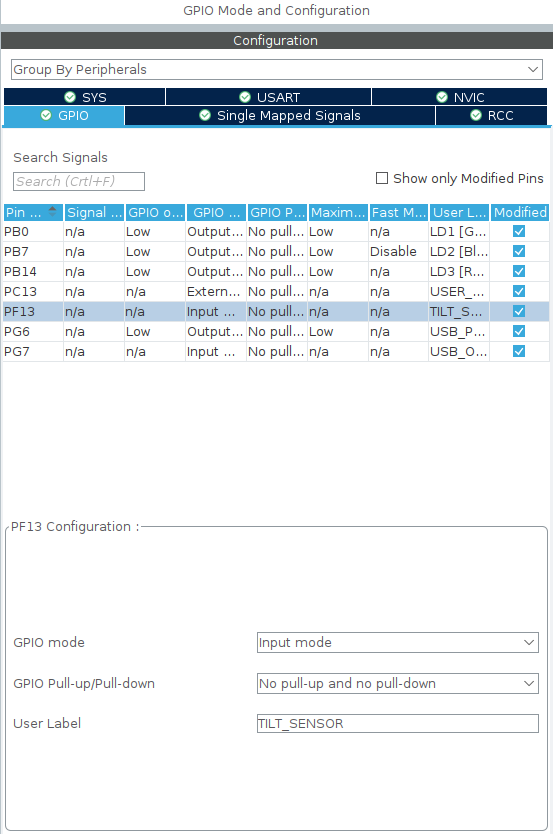
\includegraphics[width=9cm]{fig/KY-017/polaczenie_modulu/gpio.png}
    \caption{Konfiguracja pinu D7 (\texttt{PF13}), jako wejścia GPIO}
    \label{fig:gpio}
\end{figure}
\vspace{0.5cm}

\subsection{Oprogramowanie mikrokontrolera}
Kod obsługujący moduł znajduję sie w suplemencie umieszczonym pod koniec rozdziału.

\newpage

\section{Prezentacja działania układu}
Układ podłączono do mikrokontrolera z wgranym programem.

\vspace{0.5cm}
\begin{figure}[h!]
    \centering
    \includegraphics[width=9cm]{fig/KY-017/działanie_ukladu/IMG_0568.png}
    \caption{Złożony układ}
    \label{fig:smiga}
\end{figure}
\vspace{0.5cm}


Działanie układu zostało zaprezentowane na filmiku \cite{yt}, oraz na poniższym zrzucie ekranu
wyświetlającym dane odczytywane z czujnika.

\begin{figure}[h!]
    \centering
    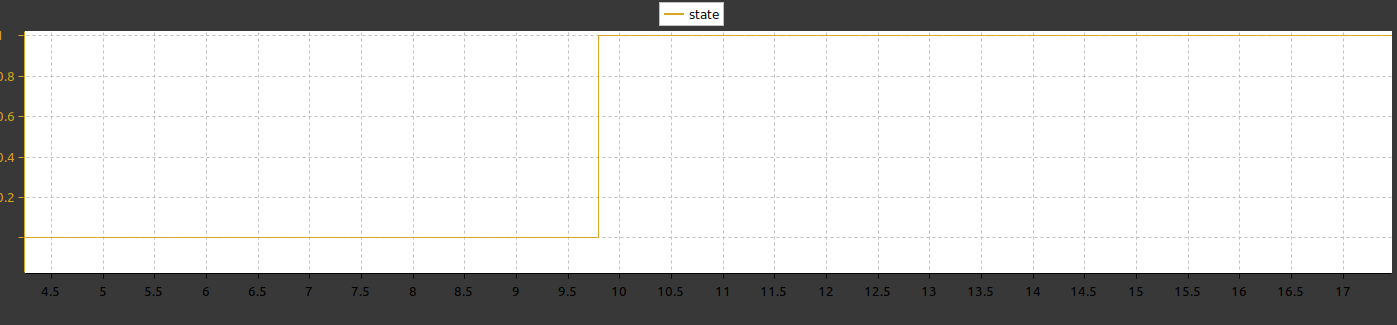
\includegraphics[width=0.8\textwidth]{fig/KY-017/działanie_ukladu/SWV.png}
    \caption{Zrzut ekranu z SWV}
    \label{fig:my_label}
\end{figure}
\vspace{0.5cm}

\printbibliography[heading=bibintoc]

\end{document}